\documentclass[./00PhotoBox.tex]{subfiles}
\graphicspath{{\subfix{./img/}}}
\begin{document}


\chapter{Photogrammetrische Grundlagen}
\label{c:photogrammetrie}
Das zu entwickelnde System soll 3D-Modelle von Objekten erstellen. Dieses Kapitel beschreibt die hierfür notwendigen Bedingungen und die Grundlagen der Rekonstruktion des Objektes als 3D-Modell. Hierfür wird Photogrammetrie in Form einer \gls{SfM}-Pipeline genutzt. Der allgemeine Ablauf ist in \autoref{img:ablauf} dargestellt. Grau dargestellte Schritte werden nicht von der entwickelten Software aus \autoref{c:software} sondern von externer Software durchgeführt.

Zunächst werden die Bilder aufgenommen (siehe \autoref{s:bilder}). Hierbei ist wichtig, dass sich die Bildinhalte überlappen. Die Bilder werden dann verknüpft, indem identische Punkte in den Bildern identifiziert werden  (siehe \autoref{s:verknuepfung}). Hierfür können beispielsweise ArUco-Marker oder die SIFT-Methode genutzt werden.
Aus den identifizierten Punkten werden dann die Positionen und Ausrichtung der Kameras und Verknüpfungspunkte in einem lokalen Koordinatensystem ohne bekannten Maßstab berechnet. Die so erzeugten Daten werden anschließend in einer Bündelblockausgleichung gemeinsam optimiert (siehe \autoref{s:buendelblock}). Durch die Nutzung von bekannten Größen, beispielsweise kalibrierten Maßstäben, kann dieses System transformiert werden.

\begin{figure}
    \centering
    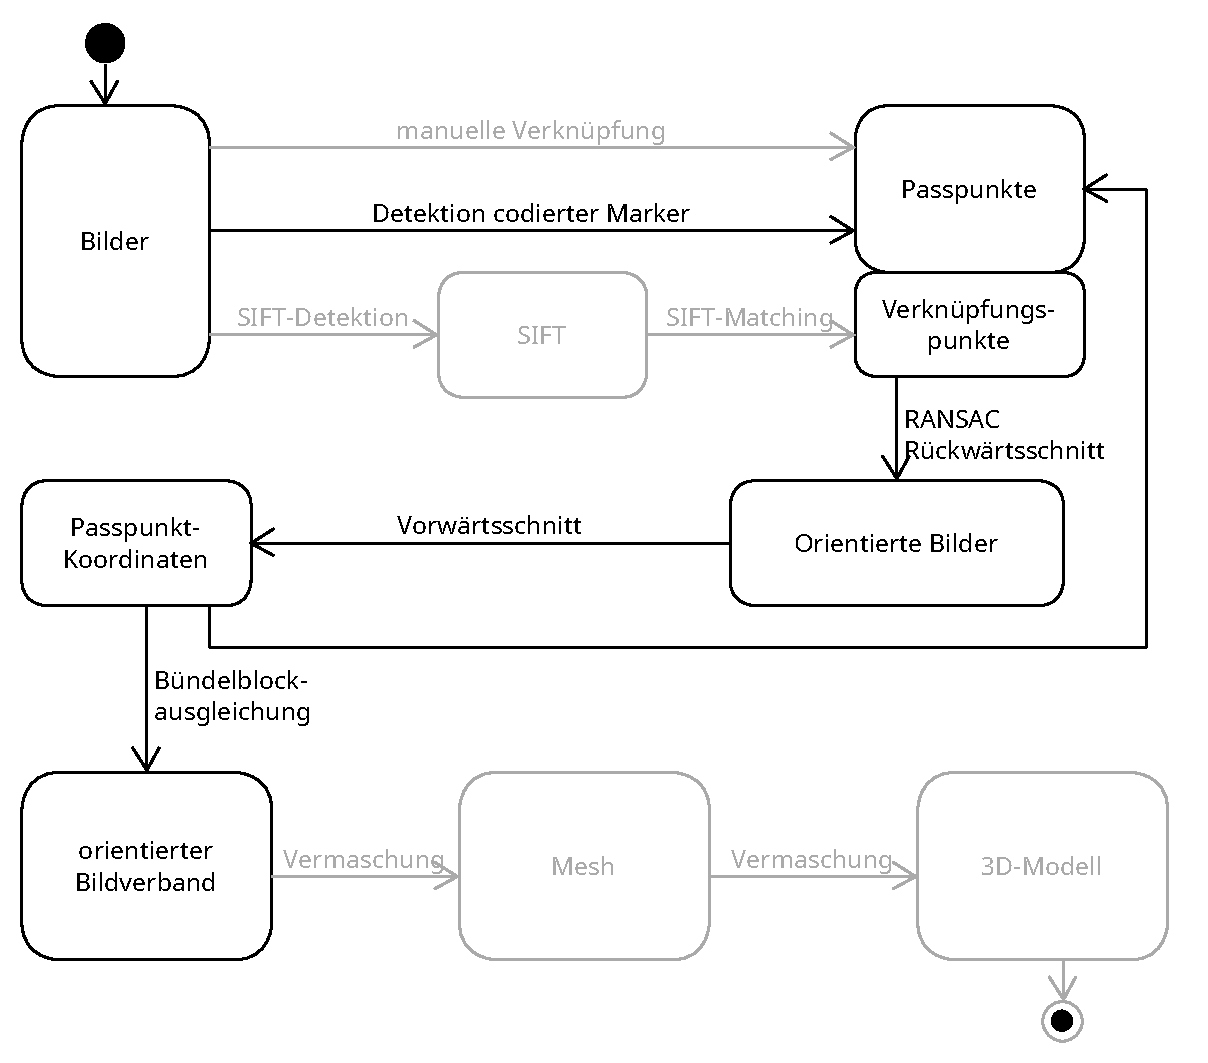
\includegraphics[width=0.8\textwidth]{./img/uml/uml_ablauf.pdf}
    \caption{Ablauf der Bildverknüpfung, nach \citealt[S. 492]{luhmann}} %Bildunterschrift
    \label{img:ablauf} %ID fürs Bild
\end{figure}



\section{Abbildung}

Grundlage der Photogrammetrie ist die Abbildungsgleichung. Diese beschreibt die Abbildung eines Punktes im Raum auf dem Sensor beziehungsweise dem Film. Umgekehrt kann mit ihrer Hilfe aus der Position eines Punktes in einem Bild, ähnlich einer Messung mit einem Theodolit, die Richtung des Punktes in Relation zu der Kamera bestimmt werden. Die Abbildungsgleichung ist abhängig von der inneren und äußeren Orientierung der Kamera. Die innere Orientierung beschreibt die Abbildungseigenschaften der Kamera, die äußere Orientierung die Position und Ausrichtung der Kamera. Im folgenden wird zuerst auf die innere und äußere Orientierung eingegangen, bevor die Abbildungsgleichung vorgestellt wird.

\subsection{Innere Orientierung}
\label{s:innereorientierung}
Die innere Orientierung beschreibt die Abbildungseigenschaften der Kamera mathematisch. Wichtigste Parameter sind hierbei die Lage des Bildhauptpunktes und die Kamerakonstante. Außerdem zählen hierzu auch die Parameter, die die Verzeichnung beschreiben. \citep[S. 179f]{luhmann}

Normalerweise wird die Kamera hierbei vereinfacht als Lochkamera unter Verwendung der Zentralperspektive betrachtet (siehe \autoref{img:optische_achse}). Als Projektionszentrum wird hierbei der Punkt beschrieben, durch den alle Bildstrahlen geradlinig laufen. Sein Lot auf dem Sensor wird als Bildhauptpunkt $H$ bezeichnet und beispielsweise durch seine Lage in Pixeln oder Mikrometern beschrieben. Durch eine schiefe optische Achse kann dieser vom Mittelpunkt des Sensors abweichen. Die Kamerakonstante $c$ beschreibt idealisiert den Abstand des Projektionszentrums zum Sensor. \citep[S. 177]{luhmann}

Als Verzeichnung wird die Abweichung der Abbildung von der idealen Lochkamera bezeichnet. Diese kann durch die Nutzung von Linsen oder durch die Bauweise der Kamera entstehen. Die Verzeichnung wird in radialer und tangentialer Verzeichnung unterschieden. Die radiale Verzeichnung beschreibt die Verzerrung der Bildpunkte in radialer Richtung, die tangentialen Verzeichnungen die Verzerrung in tangentialer Richtung. Am wichtigsten ist hierbei die radialsymmetrische Verzeichnung, da diese die größte Auswirkung hat. \citep[S. 178]{luhmann}

Jede Einstellung der Kameraoptik verändert die innere Orientierung und auch jede Kamera, selbst in derselben Modellreihe, muss je nach Genauigkeitsanspruch als unterschiedlich angesehen werden. Änderungen können sich beispielsweise durch Umfokussierung oder die Nutzung eines optischen Zoom ergeben, aber auch durch einen mechanisch instabilen Aufbau der Kameras. Daher sollten die Bilder normalerweise möglichst mit nur einer Kamera mit festen Einstellungen (Brennweite, Fokus, Blende, Objektiv) aufgenommen werden. Änderungen der Empfindlichkeit (ISO-Zahl) oder Belichtungszeit sind unproblematisch für die innere Orientierung, da hierbei die Abbildungseigenschaften der Kamera nicht verändert werden. \citep[S. 176]{luhmann}

Die Bestimmung der inneren Orientierung, auch Kalibrierung genannt, kann wäh\-rend der Messung beispielsweise als Parameter in der Bündel\-block\-ausgleichung erfolgen. Je nach Anzahl der Kameras und Stabilität der inneren Orientierung sind hier verschiedene Varianten möglich. Bei stabilen Kameras wird ein Parameter-Satz pro Kamera für eine ganze Messreihe ausgeglichen, bei instabilen Kameras kann die Kalibrierung jedes einzelnen Bildes notwendig werden. \citep[S. 181f]{luhmann}

\begin{figure}
    \centering
    \includesvg[width=0.8\textwidth]{./img/optischeAchse}
    \caption{Abbildung des Lochkamera-Modells mit Spiegelung am Projektionszentrum (rot), nach \citealt[S. 154]{hartley}, Beschriftung nach \citealt{luhmann}} %Bildunterschrift
    \label{img:optische_achse}
\end{figure}


\subsection{Äußere Orientierung}
\label{s:aeussereorientierung}
Die äußere Orientierung beschreibt die Lage der Kamera im Raum und ihre Ausrichtung. Sie wird durch die Position des Projektionszentrums und die Richtung der optischen Achse beschrieben. Die Position wird durch die Koordinaten des Projektionszentrums in einem Koordinatensystem -- in der Nahbereichsphotogrammetrie oft einem lokalen -- beschrieben. Die Richtung der optischen Achse wird mit der Rotation der Kamera beschrieben, beispielsweise durch eine Rotationsmatrix, eulersche Winkel oder Quaternionen. Durch die Nutzung von Passpunkten oder bekannten Koordinaten der Kamera kann die äußere Orientierung bestimmt werden. \citep[S. 273ff]{luhmann}

Die Darstellung der Rotation der Kamera als Quaternionen hat den Vorteil, dass diese dann mit nur vier Parametern in eine Bündelblockausgleichung eingeht. Bei der Nutzung der Rotationsmatrix hätte man hier neun bzw. acht unabhängige Parameter. Die Nutzung von eulerschen Winkeln hat den Nachteil, dass hier ein sogenannter Gimbal-Lock auftreten kann, bei dem zwei Achsen zusammenfallen und die Rotation nicht mehr eindeutig bestimmt werden kann. \citep[S. 63]{luhmann}

\subsection{Abbildungsgleichung}
\label{ss:abbildungsgleichung}
Die Abbildung eines Punktes auf einem Bild wird durch die Abbildungsgleichung beschrieben. Hierfür gibt es verschiedene Schreibweisen. In der Matrizenrechnung besteht diese aus der Multiplikation der homogenen Punktkoordinaten $X$ mit der Projektionsmatrix $P$ (\autoref{eq:abbildungsgleichung}). $P$ ergibt sich aus der Kalibrier- oder Kameramatrix $K$, der Rotation $R$ und dem Projektionszentrum $X_0$ (\autoref{eq:pkr}). Die Kalibriermatrix wiederum besteht aus der Kamerakonstante und der Lage des Bildhauptpunktes (\autoref{eq:k}).
(nach \citealp[S. 244]{hartley} und \citealp[S. 290]{luhmann})

Die äußere Orientierung ist durch die Matrix $[R|X_0]$ beschrieben (\autoref{eq:r}). Diese besteht aus der Rotationsmatrix $R$ und dem Projektionszentrum $X_0$. Die Rotationsmatrix beschreibt die Ausrichtung der Kamera im Raum, das Projektionszentrum beschreibt die Position der Kamera bzw. des Projektionszentrums im Raum.

\begin{align}
    \label{eq:abbildungsgleichung}
    x'      & = P \cdot X       \\
    \label{eq:pkr}
    P       & = K \cdot [R|X_0] \\
    \label{eq:k}
    K       & =
    \begin{bmatrix}
        c_x & 0   & x'_0 \\
        0   & c_y & y'_0 \\
        0   & 0   & 1    \\
    \end{bmatrix}            \\
    \label{eq:r}
    [R|X_0] & =
    \begin{bmatrix}
        r_11 & r_21 & r_31 & X_0 \\
        r_12 & r_22 & r_32 & Y_0 \\
        r_13 & r_23 & r_33 & Z_0 \\
    \end{bmatrix}
\end{align}
\begin{conditions}
    x' & Bildkoordinate \\
    P  & Projektionsmatrix \\
    X  & Homogene Punktkoordinaten \\
    K  & Kalibrier- oder Kameramatrix \\
    R  & Rotationsmatrix \\
    X_0 & Projektionszentrum \\
    c_x, c_y & Kamerakonstante in x- und y-Richtung \\
    x'_0, y'_0 & Lage des Bildhauptpunktes in x- und y-Richtung \\
    r_{...} & Parameter der Rotationsmatrix \\
\end{conditions}

% Um die Beziehung zwischen zwei Bildern aufzustellen, kann man diese Abbildungsgleichung nutzen. Da es hier nur um die Beziehung zwischen zwei Bildern geht, kann die Rotation und Translation des ersten Bildes auf 0 gesetzt werden ($R$ ist dann eine 3x3-Einheitsmatrix und $X_0$ ein Nullvektor). $X_0$ des zweiten Bildes wird zur Translation zwischen den beiden Bildern. \citep[S. 330]{luhmann}

Grundlage dieser Formel ist das Lochkamera-Modell (siehe \autoref{img:optische_achse}). Dabei wird rechnerisch das Bild an dem Projektionszentrum in den Objektraum gespiegelt (rot im Bild). Dadurch kann mit einem aufrechten Bild gerechnet werden.

Als weitere Parameter spielen die Verzeichnungen eine Rolle. Diese kann in die Abbildungsgleichung integriert werden, in dem $x'$ durch $\Delta x'$ korrigiert wird. \citep[S. 277]{luhmann}

\begin{align}
    \label{abbildungsgleichung_verzerrung}
    x'        & = P \cdot X + \Delta x'                 \\
    \Delta x' & = \Delta x_{rad} + \Delta x_{tan} + ...
\end{align}
\begin{conditions}
    \Delta x' & Verzeichnung \\
    \Delta x_{rad} & Radiale Verzeichnung \\
    \Delta x_{tan} & Tangentiale Verzeichnung \\
\end{conditions}

Die Verzeichnungen werden meist mit den Parametern $k1$ bis $k4$ für die radiale Verzeichnung und $p1$ und $p2$ für die tangentialen Verzeichnungen bezeichnet. Die Faktoren stellen dabei die Parameter einer Taylor-Reihe dar. Sie basieren auf dem Kameramodell von Brown und den von ihm in \cite[S. 859]{brown1971} vorgestellten Formeln (siehe \autoref{eq:brown_rad} und \ref{eq:brown_tan}).

\begin{align}
    \label{eq:brown_rad}
    \Delta x_{rad} = k1 \cdot r^2 + k2 \cdot r^4 + k3 \cdot r^6 + k4 \cdot r^8 \\
    \label{eq:brown_tan}
    \Delta x_{tan} = 2 \cdot p1 \cdot x \cdot y + p2 \cdot (r^2 + 2 \cdot x^2)
\end{align}
\begin{conditions}
    r & Abstand des Punktes zum Bildhauptpunkt \\
    x & Bild-x-Koordinate des Punktes \\
    y & Bild-y-Koordinate des Punktes \\
    k1, k2, k3, k4 & Radiale Verzeichnungsparameter \\
    p1, p2 & Tangentiale Verzeichnungsparameter \\
\end{conditions}

Diese Parameter werden beispielsweise auch in Metashape, OpenDroneMap und OpenCV genutzt.


\section{Bilder}
\label{s:bilder}

Die Berechnung der Position eines Objektes im Bild ist nur möglich, sofern der Punkt in mindestens einem weiteren Bild abgebildet ist. Die Genauigkeit der Berechnung ist vom Schnittwinkel dieser beiden Strahlen abhängig. Um möglichst gute Grundlagen zur Ver\-fügung zu haben und die innere und äußere Orientierung möglichst gut berechnen zu können, müssen diese Bilder einige Bedingungen erfüllen - auf diese wird hier eingegangen.

\subsection{Überlappung und Bildinhalte}
Da die Bilder durch identische Punkte verbunden werden, müssen sich die Bildinhalte überlappen und gemeinsame Punkte in den Bildern identifiziert werden. Die automatische Detektion von identischen Punkten ist auf verschiedene Weisen möglich: Entweder durch die Nutzung von codierten und uncodierten Passpunkten oder über eine Merkmalsextraktion. Für das letztere muss die Oberfläche genügend Textur bzw. Struktur aufweisen. Detailliert wird in \autoref{s:verknuepfung} hierauf eingegangen. \citep[S. 478]{luhmann}

\subsection{Position und Ausrichtung der Kamera}
Damit die Schnitte der Bildstrahlen optimal sind und die Berechnung der Tiefeninformationen möglichst genau ist, müssen die Kameras möglichst gleichmäßig um das Objekt verteilt sein.
Bilder, die vom gleichen Standpunkt aufgenommen wurden, sind oft nur ungenau verknüpfbar. Daher empfiehlt es sich, Bilder aus verschiedensten Richtungen zu machen, also bei der manuellen Photographie um das Objekt herumzugehen - eine Mehrbildaufnahme im Rundum-Verband zu erzeugen. \citep[S. 170]{luhmann}

Entsprechend müssen die Kameras gleichmäßig um das Objekt verteilt positioniert werden und dabei auch an die Form des Objektes wie Einschnitte anpassbar sein.

\subsection{Belichtung}
Um identische Punkte in den Bildern identifizieren zu können, müssen die Bilder eine gleichmäßige Beleuchtung aufweisen. Hierfür sollte es vermieden werden, dass Schatten auf das Objekt fallen. Eine gleichmäßige Beleuchtung kann durch die Nutzung von mehreren Lichtquellen erreicht werden. Auch sollte keine Blendwirkung entstehen, die durch direkte Sonneneinstrahlung oder Reflexionen entstehen kann. Die Belichtung der einzelnen Bilder sollte möglichst identisch sein, damit später auch eine zusammenhängende Texturierung möglich ist.
Da die Objekte und die Kameras sich während der Aufnahme nicht bewegen, kann die Belichtungszeit verlängert werden, um Rauschen durch eine zu hohe Sensorempfindlichkeit zu vermeiden und so die Bildqualität zu erhöhen.


\subsection{Fokussierung und Schärfentiefe}
\label{s:schaerfe}
Um genaue Punktwolken zu ermöglichen, muss das Objekt scharf abgebildet werden. Die Kameras müssen dafür entsprechend fokussiert sein. Jedoch wird durch die Fokussierung auch die innere Orientierung verändert. Normalerweise wird daher auf eine Umfokussierung verzichtet und mittels der Blende (kleine Blendenöffnung) die Schärfentiefe erhöht, sodass ein großer Bereich scharf abgebildet wird. Dieses ist aber bei vielen einfachen Kameras wie dem verwendeten Raspberry Pi Camera Module 3 nicht möglich.

Der Schärfebereich ergibt sich aus der Größe des tolerierbaren Unschärfekreis auf dem Sensor. Bei digitalen Kameras wird dieser durch die Pixelgröße bestimmt. Nach \citet[S. 148f]{luhmann} berechnet sich die Schärfentiefe nach folgender Formel:

\begin{align}
    \label{eq:schaerfebereich}
    t   & = a_h - a_v            \\
    a_v & = \frac{a}{1+K}        \\
    a_h & = \frac{a}{1-K}        \\
    K   & = \frac{k(a-f)u'}{f^2}
\end{align}
\begin{conditions}
    t   & Länge des Schärfebereich \\
    a_v, a_h & Vordere bzw. hintere Grenze der Schärfentiefe\\
    a   & Fokussierte Dingweite\\
    k   & Blendenzahl\\
    f   & Brennweite
\end{conditions}

Die Schärfentiefe des Raspberry Pi Camera Module 3 ist in \autoref{img:sschaerfentiefe_plot} für einen Unschärfekreis von drei Pixeln dargestellt (Plot der \autoref{eq:schaerfebereich}). Es zeigt sich, dass die Schärfentiefe im  verwendeten Makrobereich relativ klein ist. Problematisch ist dies vorallem bei größeren Objekten, die hierdurch näher an die Kameras rücken, aber durch ihre Größe einen größere Schärfentiefe benötigen. Ein Lösungsansatz durch Kombination mehrere Aufnahmen wird in \autoref{sec:fokusstacking} untersucht.

\begin{figure}
    \centering
    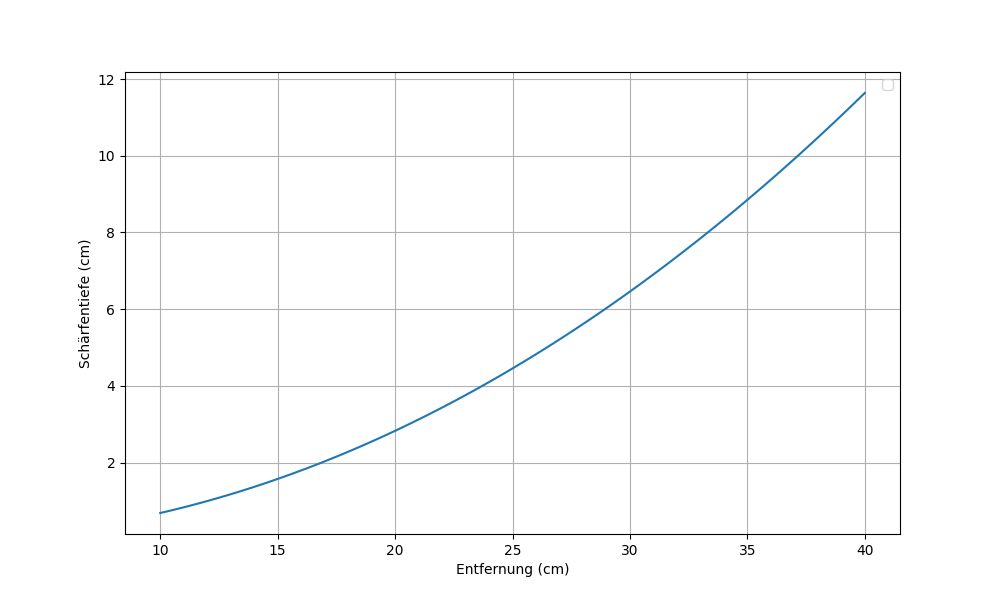
\includegraphics[width=0.9\textwidth]{./img/schaerfentiefe_plot.png}
    \caption{Schärfentiefe in Abhängigkeit von der fokussierten Entfernung} %Bildunterschrift
    \label{img:sschaerfentiefe_plot} %ID fürs Bild
\end{figure}


\section{Skalierung/Maßstab}
\label{sec:massstab}
Die Skalierung eines rein photogrammetrisch bestimmten 3D-Modelles ist nicht bekannt, da die Berechnungen nur auf Richtungen ohne Längenangaben basieren. Daher werden Referenzen in Form einer bekannten Länge benötigt, um die Skalierung zu bestimmen. Alternativ können auch Passpunkte (siehe \autoref{s:verknuepfung}) mit bekannten Koordinaten verwendet werden oder im Falle von Mehrkamerasystemen bekannte äußere Orientierungen der Kameras. \citep[S. 546]{luhmann}


\section{Verknüpfungs- und Passpunkte}
\label{s:verknuepfung}
Um die einzelnen Bilder verknüpfen zu können, werden identische Punkte zwischen zwei oder mehr Bildern benötigt. Diese können klassisch manuell erfasst werden, jedoch ist dieses schon bei kleineren Projekten sehr zeitaufwändig. Daher wird meist die Möglichkeit genutzt, automatisch Verknüpfungspunkte zu erzeugen. Hierfür gibt es unterschiedliche Methoden, die im Folgenden vorgestellt werden.


\subsection{Zielmarker}
Es gibt verschiedenste Formen von Markern, die automatisch erfasst werden können. Grob unterschieden werden kann in codierte und nicht codierte Zielmarker. Beispiele für nicht codierte sind beispielsweise einfache kreisförmige Klebepunkte oder Marker, die aus Linien bestehen und ihren Mittelpunkt durch dessen Schnitt definieren.
Vorteilhaft ist jedoch die Verwendung von codierten Zielmarken. Hier können die Punkte direkt zugeordnet werden, sodass keine weitere Filterung und Berechnung zur Zuordnung notwendig ist. \citep[S.535ff]{luhmann}

\subsubsection{Zielmarken nach Schneider}
Eine Form der codierten Zielmarken sind die Marker nach Schneider. Diese bestehen aus mehreren konzentrischen Kreisen und werden entsprechend auch als CCCT -- concentric circular coded target -- bezeichnet \citep{ccct}. Die Mitte des Markers wird durch den gemeinsamen Mittelpunkt der Kreise definiert.  Vorteilhaft ist, dass die Marker auch bei unscharfen Bildern erkannt werden können und ihr Zentrum manuell identifiziert werden kann, beispielsweise zum Aufmaß mit einem Tachymeter. Sie haben sich daher als Standardmarker in der Photogrammetrie etabliert. Sie werden beispielsweise von Agisoft Metashape verwendet.
\todo{Quelle}


\subsubsection{ArUco-Marker}
Eine andere Variante der codierten Verknüpfungspunkte sind die sogenannten ArUco-Marker. Diese werden häufig für die Orientierung bei Augmented-Reality-An\-wend\-ungen genutzt. Sie werden als codierte Messmarken verwendet und können automatisch im Subpixelbereich erkannt werden. Jede Ecke kann hier einzeln identifiziert werden, sodass ein erkannter Marker vier Verknüpfungspunkte liefern kann. Nachteilig ist, dass die Ecken nicht eindeutig identifiziert werden können, wenn die Aufnahme unscharf ist. Durch ihre Verwendung in Augmented-Reality-Anwendungen sind auch viele kostenfreie Bibliotheken für ihre Erkennung verfügbar. Beispielsweise kann OpenCV ArUco-Marker identifizieren. %\citep[S. 536]{luhmann}
\todo{Quelle}

\subsection{Merkmalsextraktion}
Ohne das Anbringen von Markern können auch Merkmale in den Bildern erkannt werden. Hierfür gibt es verschiedene Methoden, eine dieser ist die SIFT-Methode, welche hier beispielhaft kurz dargestellt wird. Sie liefert Verknüpfungspunkte aus Mustern auf den photographierten Oberflächen. Es ist meist nicht notwendig explizit Marker an dem aufzunehmenden Objekt anzubringen, sofern seine Oberfläche nicht strukturlos ist (glatte weiße Wände etc.) oder in Bewegung ist.

Zur Erkennung von Merkmalen setzt das Verfahren auf die Detektion von Kanten. Diese werden in verschiedenen Stufen einer Bildpyramide erkannt und ihre Extrema berechnet. Sie werden anschließend weiter ausgedünnt, beispielsweise über den Kontrast. Sofern ein möglicher Marker identifiziert wurde, wird eine Beschreibung erzeugt. Diese erfolgt  durch Analyse der Helligkeitsabweichungen zu den Nachbar-Pixeln und wird an der stärksten Abweichung ausgerichtet. Hierdurch wird die Beschreibung dann richtungsunabhängig. Mit diesen kann dann die Übereinstimmung von zwei Markern in zwei Bildern bestimmt werden, auch wenn diese zueinander gekippt oder gedreht sind.
\citep[S. 484f]{luhmann}

\section{Verknüpfung von Bildern}
\label{s:photogramm}
Durch die beschriebenen Verfahren und die hieraus entstandenen Verknüpfungs\-punkte können die Bilder miteinander verknüpft werden. Da die Kamerapositionen am Rahmen veränderlich sind und die Montage auch keine ausreichend genaue Fixierung garantiert, können die bekannten Positionen aus vorherigen Messungen maximal als Näherungswerte genutzt werden. Die genaue Bestimmung der Position und Ausrichtung - die äußere Orientierung - muss daher mindestens für die verschobenen oder gedrehten Kameras neu berechnet werden. Gleiches gilt für neue Verknüpfungspunkte, für die noch keine Koordinate bekannt ist. Die beiden Verfahren, die so zur Verknüpfung der Bilder beitragen, werden im Folgenden vorgestellt.


\subsection{Rückwärtsschnitt}
Sofern Koordinaten von Passpunkten bekannt sind, können die Positionen und Ausrichtungen der Kameras berechnet werden. Hierfür wird der sogenannte Rückwärtsschnitt genutzt. Die Berechnung erfolgt auf Basis der Abbildungsgleichung, die die Position eines Punktes in einem Bild in Beziehung zur Kamera setzt. Für die Berechnung selbst gibt es verschiedene Methoden. Verwendet wurde hier der von OpenCV genutzte Ansatz von \citeauthor{Lepetit2008} in Kombination mit einem RANSAC-Ansatz. Durch die Nutzung des RANSAC-Ansatzes können veränderte Passpunkte identifiziert und als Ausreißer markiert werden.

\todo{Bild + Erklärung}

\subsection{Vorwärtsschnitt}
Um wiederum aus einem Stereopaar mit bekannter innerer und äußerer Orientierung Punktkoordinaten zu berechnen, wird der Vorwärtsschnitt genutzt. Hierfür sind die Bildkoordinaten des zu berechnenden Punktes in beiden Bildern notwendig.

Mit dem Vorwärts\-schnitt können neben markierten Verknüpfungspunkten auch die Neupunkte, die mittels SIFT oder ähnlichen Bild\-erkennungs\-algorithmen erkannt wurden, berechnet werden. Dadurch kann eine dünne Punktwolke erzeugt werden.

\begin{comment}
Die Koordinaten der Passpunkt-Ausreißer aus der Berechnung der Kamerapositionen werden anschließend neu berechnet. Hierfür wird der Vorwärtsschnitt genutzt. Auch hier wird OpenCV zur Berechnung genutzt. Die Berechnung der Passpunkte erfolgt für jedes Bildpaar einzeln. Für alle Koordinaten wird dann pro Passpunkt der Z-Score berechnet. Passpunkte, die einen Z-Score von über 2 haben, werden als Ausreißer markiert und nicht weiter betrachtet.
\end{comment}
\todo{Bild + Erklärung}

\section{Bündelblockausgleichung}
\label{s:buendelblock}
Mittels Bündelblockausgleichung können die grob mit den vorher genannten Verfahren bestimmten Positionen und Drehungen in einer Ausgleichung optimiert werden. Hierzu gehen alle Parameter der Bilder und die Positionen der Passpunkte in die gemeinsame Ausgleichung ein. Grundlage der Ausgleichung ist die in \autoref{ss:abbildungsgleichung} beschriebene Abbildungsgleichung. Als Ergebnis erhält man die ausgeglichenen Parameter und Genauigkeitsangaben für diese. \citep[S. 343ff]{luhmann}

Neben der Optimierung der Parameter hat die Bündelblockausgleichung auch den Vorteil, dass instabile Kameras, wie sie in diesen Projekt verwendet werden, simultan kalibriert werden können. Hierbei werden die inneren und äußeren Orientierungen der Kameras gemeinsam optimiert. Die in vorherigen Untersuchungen festgestellten, jedoch nicht genauen Parameter der Kamera werden hierbei als Näherungswerte genutzt und die endgültigen Parameter erst durch die Ausgleichung bestimmt. Es ist daher unkritisch, wenn sich die Parameter der Kamera im geringen Rahmen zwischen den Aufnahmen verändern. \citep[S. 357f]{luhmann}


\section{Multi-view Stereo}
Die dünne Punktwolke aus dem Vorwärtsschnitt und der anschließenden Bündel\-block\-ausgleichung kann durch das Multi-view Stereo-Verfahren zu einem 3D-Modell erweitert werden. Hierbei werden jeweils Bildpaare gebildet und die Disparitäten, also die Verschiebung des Objektes in der Abbildung, bestimmt. Diese sind abhängig von der Entfernung des Objektes. Bei einem unendlich weit entfernten Objekt tritt keine Disparität auf \citep[S. 313]{luhmann}. Die Disparitäten können dann in Tiefeninformationen umgerechnet, gemittelt und zu einem Tiefenbild zusammengefasst werden. \citep[S. 505]{luhmann}
%\citep[S. 51]{opendronemap}

\section{Mesh-Generierung}
Bis zu diesem Schritt besteht das Modell nur aus einzelnen Punkten, die keine Oberfläche ergeben. Um ein geschlossenes 3D-Modell zu erhalten, muss eine Oberfläche generiert werden. Hierfür wird ein Mesh-Generierungsverfahren genutzt, welches die Punktwolke in Dreiecke unterteilt. Es gibt verschiedene Verfahren, die sich in der Art der Unterteilung und ihrem Umgang mit Einzelpunkten unterscheiden. OpenDroneMap nutzt beispielsweise die Screened Poisson Surface Reconstruction. \citep[S. 52f]{opendronemap}

Die Screened Poisson Surface Reconstruction ist ein Verfahren, das auf der Poisson-Gleichung basiert. Diese wird genutzt, um die Oberfläche zu glätten und zu interpolieren. Ein Teil des Ansatzes ist es, die Ausrichtung der Punkte zu berücksichtigen. Die Punkte werden hierbei in eine Gitterstruktur überführt und die Oberfläche durch die Lösung der Poisson-Gleichung bestimmt. \citep{spsr}
\todo{Details zur Poisson-Gleichung}

\section{Texturierung}
Abschließend wird das Modell texturiert. Hierfür werden die Bilder, die zur Erstellung des Modells genutzt wurden, auf das Modell projiziert. Außerdem werden Helligkeits- und Farbunterschiede ausgeglichen. \citep[S. 54f]{opendronemap}
\todo{erweitern}

\biblio
\end{document}